\documentclass[10pt,a4paper]{article}
\usepackage{verbatim}
\usepackage{subcaption}
\usepackage{karnaugh-map}
\usepackage[utf8]{inputenc}
\usepackage[italian]{babel}
\usepackage{amsmath}
\usepackage{amsfonts}
\usepackage{amssymb}
\usepackage{graphicx}
\usepackage[left=2cm,right=2cm,top=2cm,bottom=2cm]{geometry}
\newcommand{\rem}[1]{[\emph{#1}]}
\newcommand{\exn}{\phantom{xxx}}
\renewcommand{\thesubsection}{\thesection.\alph{subsection}}  %% use 1.a numbering

\author{Gruppo EB.24 \\Giovanni Sucameli, Davide Incalza, Francesco Sacco}
\title{Effetto fotoelettrico - Misura del rapporto $\frac{h}{e}$}
\begin{document}
\date{25 Marzo 2019}
\maketitle
\section*{Scopo dell'esperienza e cenni teorici}
Obiettivo di questa esperienza è la verifica dell'effetto fotoelettrico e dell'ipotesi di Einstein formulata nel 1905 e successivamente verificata da Millikan, secondo cui un'onda elettromagnetica è costituita da quanti di luce, detti fotoni, ciascuno dei quali porta un energia 

\begin{equation}
E_{\gamma} = h\nu
\label{energia}
\end{equation}
dove h è la costante di Planck e $ \nu $ la frequenza dell'onda. Affinchè un elettrone venga estratto dal metallo è necessario che assorba un fotone di energia superiore al lavoro $ W_{0}$ di estrazione dal metallo ( $ W_{0} $)  varia da metallo a metallo). Dunque l'energia cinetica del fotoelettrone è data da
\begin{equation}
    E_{e} = hv - W_{0}
\label{foto}
\end{equation}
Da quest'ultima equazione ricaveremo poi anche una stima del rapporto $ \frac{h}{e} $
Notiamo infine che, secondo l'ipotesi di Einstein, l'intensità della corrente formata dai fotoelettroni è proporzionale al numero di fotoni (con energia tale da estrarre l'elettrone dal metallo) incidenti sul metallo nell'unità di tempo.

\section*{Materiale occorrente}

\begin{itemize}
\item una lampada a led
\item una fotocella Leybold 55877 
\item filtri interferenziali (Newport)
\item scatola metallica
\item generatore di tensione continua
\item un multimetro digitale
\item un picoamperometro digitale
\end{itemize}

\section*{Esperimento di Millikan}
Robert Millikan (che già nel 1909 aveva misurato la carica elementare) tra il 1914 ed il 1916 effettuò misure per verificare l'ipotesi di Einstein. L'idea di Millikan è quella di far incidere della luce di frequenza $\nu$ (che può essere variata) su un bulbo di vetro su cui era stato depositato a vuoto un catodo alcalino. La corrente dovuta ai fotoelettroni poteva essere misurata mediante un mllliamperometro chiuso su un generatore di tensione continua in grado di generare una d.d.p. continua tra il catodo e l'anodo; la polarità è tale da generare nel bulbo un campo elettrico opposto al flusso dei fotoelettroni verso l'anodo, in modo di diminuire la corrente nel circuito. Regolando la tensione V fino ad un valore $V_{0}$ tale da annulare la corrente, si ottiene una stima dell'energia cinetica massima dei fotolettroni da mettere in relazione alla frequenza della luce (per verificare la linearità della relazione energia-frequenza (equazione \ref{foto}), e ottenere una stima del rapporto $\frac{h}{e}$ ). 
%\newline \newline
\section*{Apparato sperimentale}
Per la verifica dell'equazione (\ref{foto}) abbiamo utilizzato un metodo simile a quello usato da Millikan. L'apparato sperimentale è composto da :

\begin{itemize}
\item una fotocella Leybold 55877
\item una lampada a led usata come sorgente di luce con uno spettro quasi continuo
\item un set di filtri interferenziali con cui variare la frequenza dell'onda incidente sul catodo (i valori delle lunghezze d'onda centrali e delle bande passanti sono in Tab.\ref{tab:filtri} )
\item un generatore di tensione continua (da banco) per variare la tensione di bias tra catodo e anodo
\item un voltmetro digitale per misurare la tensione di bias all'uscita del generatore
\item un picoamperometro per misurare la corrente dei fotoelettroni
\end{itemize}


Il circuito elettrico equivalente montato nel nostro apparato sperimentale è mostrato in Fig.\ref{fig:cireq}. L'apparato è messo dentro una scatola metallica al fine di schermarlo da eventuali rumori elettromagnetici (sia la luce stessa della stanza ad esempio, che il rumore elettrico ambientale). 
Sulla scatola sono montati due connettori coassiali LEMO ( K e A) per realizzare le dovute connessioni al catodo e all'anodo.
L'ottica del banco è invece composta da :

\begin{itemize}
\item una fenditura realizzata con diaframma circolare, posta immediatamente a valle della lampada che ha lo scopo di concentrare il raggio luminoso in modo che abbia dimensioni molto inferiori al raggio dell'anodo (composto da un anello di Platino)
\item due lenti convergenti, con fuochi rispettivamente nel foro del diaframma e nel centro del fotocatodo; la loro funzione è rispettivamente quella di fare in modo che la luce che esce dal diaframma incida in modo normale sul filtro in modo da non variare la frequenza trasmessa e quella di mettere a fuoco al centro del catodo l'immagine del diaframma.
\item un setto oscuro che separi la sorgente di luce dalla fotocella 
\end{itemize}

Lo schema del banco ottico è mostrato in Fig. \ref{fig:schemabanco}.

%AGGIUNGERE QUALCOSA SUGLIO ERRORI SISTEMATICI ???????
%FINIREFINIREFINIREFINIREFINIRE....
\begin{table}[h]
\caption{\small Lunghezza d'onda centrali, rispettive frequenze con incertezze di banda associate e colore della luce in uscita per i filtri utilizzati. }
\label{tab:filtri}
\begin{center}
\begin{tabular}{c|cccc}
\hline
colore & $\lambda$ (nm) & FWHM (nm) & $\nu (10^{14} $ Hz ) & d$\nu$   \\ 
\hline
azzurro & 450.9 & 9.6 & 6.6 & 0.1\\
verde-azzurro & 499.05 & 11.10 & 6.0 & 0.1\\
verde & 546.03  & 11.68 & 5.5 & 0.1\\
giallo & 577  &  10 & 5.1 & 0.1 \\
\hline
\end{tabular}
\end{center}
\end{table}

\begin{figure}[h]
\begin{center}
\includegraphics[width=0.5\linewidth]{immagini/circuito_equivalente.png}
\caption{\small Schema elettrico equivalente per la misura dell'energia cinetica dei fotoni. }
\label{fig:cireq}
\end{center}
\end{figure}

\begin{figure}[h]
\begin{center}
\includegraphics[width=0.5\linewidth]{immagini/schema_banco.png}
\caption{\small Schema del banco ottico. }
\label{fig:schemabanco}
\end{center}
\end{figure}

\newpage
\section*{Analisi Dati}
%scrivere qualcosa su come fatto il fit ecc... qui
Il fit è stato effettuato supponendo che la relazione tra la fotocorrente $I$ e il voltaggio ai capi del catodo e l'anodo $V$ è descritta dall'equazione $I=a(V_0-V)^2\theta(V_0-V)+bV+I_0$.\newline
%grafico dei residui se li emttiamo andrebbero onormalizzati, ricorda che forti ha detto che metterle così nn hanno molto senso..chi2 scritto con 10^1 è troppo bello...
Il grafico dei residui mostra gli errori efficaci $\sigma_{eff}=\sqrt{(\sigma I)^2+[(\sigma V) \frac{dI}{dV}]^2}$
%\captionof{figure}....
Sotto, rispettivamente nelle Fig. \ref{fig:450} - \ref{fig:577} e nelle rispettive tabelle sono mostrati, per ogni frequenza selezionata, i risultati dei fit per la stima di $V_{0}$, mentre in Fig. \ref{fig:fit} e Tab. \ref{tab:fit} è mostrato il risultato per il fit per la stima di $\frac{h}{e}$.    \newline \newline


\begin{minipage}{.6\linewidth}
		\centering
		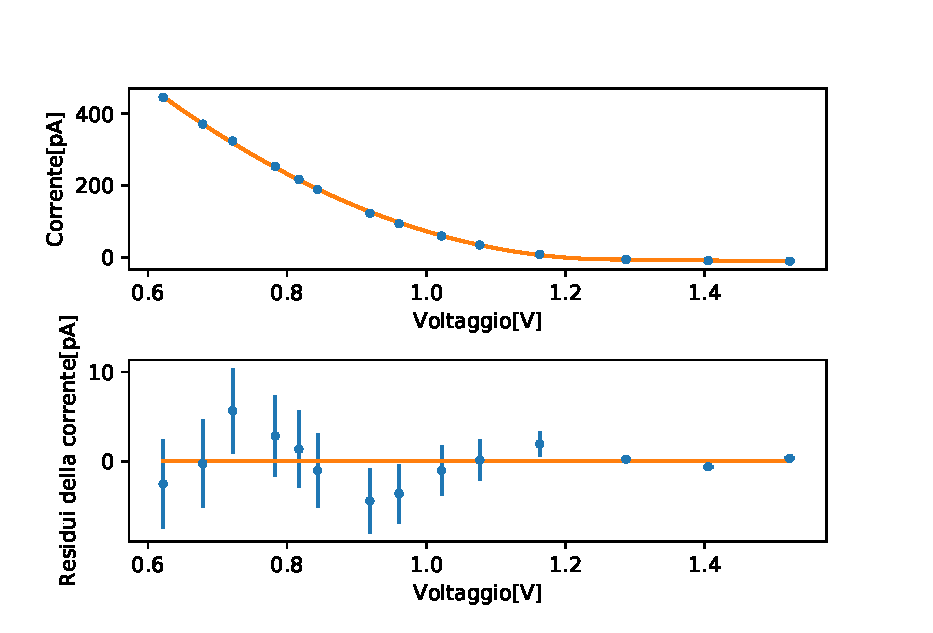
\includegraphics[width=\linewidth]{immagini/450nm.eps}
		\captionof{figure}{Grafico di best fit e dei residui a sinistra, parametri ottimali di best fit e valore del $\chi^{2}$ a destra per il filtro con banda passante centrata attorno a 450nm.  }
		\label{fig:450}
	\end{minipage}
	\begin{minipage}{.4\linewidth}
		\begin{tabular}{cc}
\hline
	Parametri di Fit & Valori di Fit\\ 
\hline
	$V_0$ & $1.26\pm0.006$ \\
	$a$ & $(-1.08\pm0.03)\times 10^{-9}$ \\
	$b$ & $(2.0\pm0.2)\times 10^{-11}$ \\
	$I_0$ & $(-2.0\pm0.2)\times 10^{-11}$ \\
	$\chi^2$ & $23.88$ \\
\hline
\end{tabular}

		\label{tab:450}
\end{minipage}\newline\newline

%RISOLVERE THIS PROBLEM......


\begin{minipage}{.6\linewidth}
		\centering
		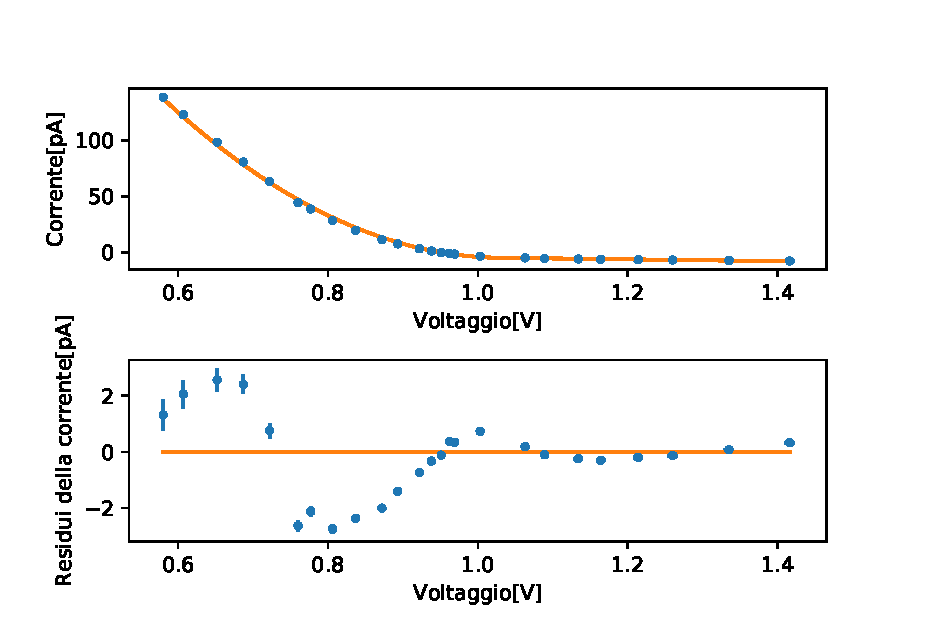
\includegraphics[width=\linewidth]{immagini/499nm.eps}
		\captionof{figure}{Grafico di best fit e dei residui a sinistra, parametri ottimali di best fit e valore del $\chi^{2}$ a destra per il filtro con banda passante centrata attorno a 499nm.}
		\label{fig:499}
	\end{minipage}
	\begin{minipage}{.4\linewidth}
		\begin{tabular}{cc}
\hline
	Parametri di Fit & Valori di Fit\\ 
\hline
	$V_0$ & $1.029$ $\pm$ $0.002$ \\
	$a$ & $(-6.9$ $\pm$ $0.1)\times 10^{-10}$ \\
	$b$ & $(8.0$ $\pm$ $0.4)\times 10^{-12}$ \\
	$I_0$ & $(-3.5$ $\pm$ $0.4)\times 10^{-12}$ \\
	$\chi^2$ & $6.43\times 10^{1}$ \\
\hline
\end{tabular}

		\label{tab:499}
\end{minipage}\newline\newline

\begin{minipage}{.6\linewidth}
		\centering
		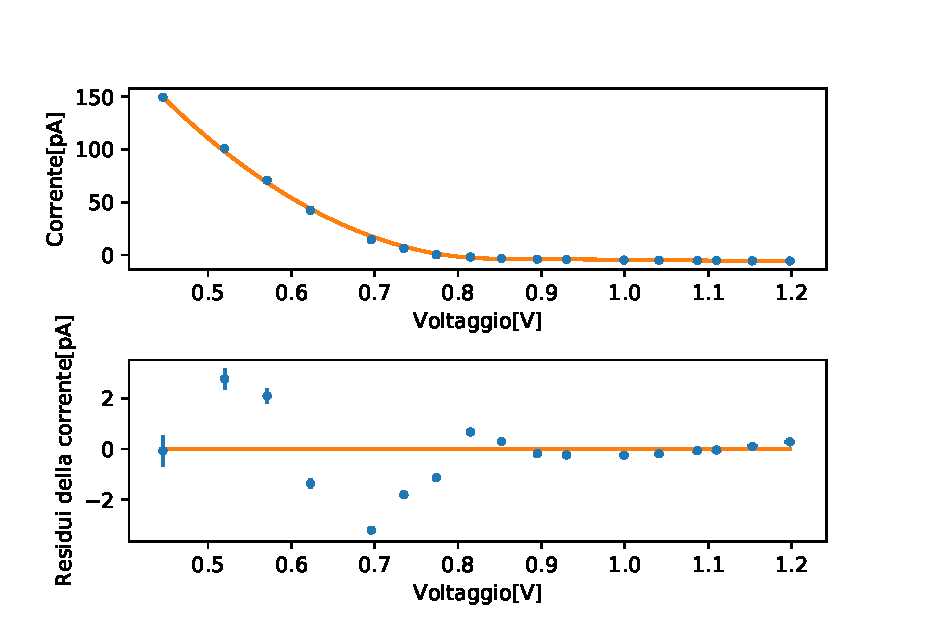
\includegraphics[width=\linewidth]{immagini/545nm.eps}
		\captionof{figure}{Grafico di best fit e dei residui a sinistra, parametri ottimali di best fit e valore del $\chi^{2}$ a destra per il filtro con banda passante centrata attorno a 545nm.}
		\label{fig:545}
	\end{minipage}
	\begin{minipage}{.4\linewidth}
		\begin{tabular}{cc}
\hline
	Parametri di Fit & Valori di Fit\\ 
\hline
	$V_0$ & $0.841$ $\pm$ $0.002$ \\
	$a$ & $(-9.7$ $\pm$ $0.2)\times 10^{-10}$ \\
	$b$ & $(7.1$ $\pm$ $0.3)\times 10^{-12}$ \\
	$I_0$ & $(-2.4$ $\pm$ $0.3)\times 10^{-12}$ \\
	$\chi^2$ & $61.8$ \\
\hline
\end{tabular}

		\label{tab:545}
\end{minipage}\newline\newline
\newline

\begin{minipage}{.6\linewidth}
		\centering
		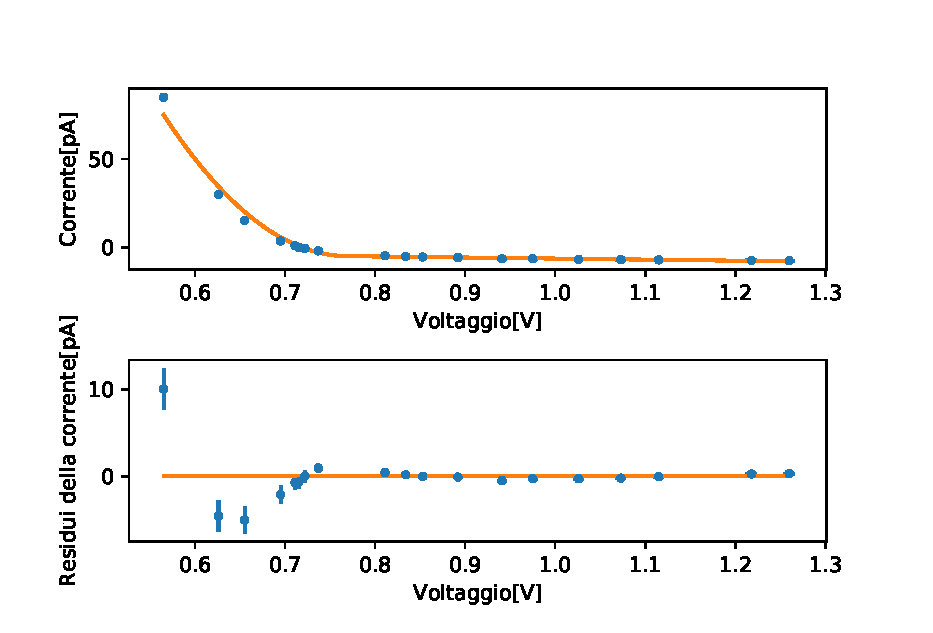
\includegraphics[width=\linewidth]{immagini/577nm.eps}
		\captionof{figure}{Grafico di best fit e dei residui a sinstra, parametri ottimali di best fit e valore del $\chi^{2}$ a destra per il filtro con banda passante centrata attorno a 577nm.}
		\label{fig:577}
	\end{minipage}
	\begin{minipage}{.4\linewidth}
		\begin{tabular}{cc}
\hline
	Parametri di Fit & Valori di Fit\\ 
\hline
	$V_0$ & $0.759\pm0.01$ \\
	$a$ & $(-2.2\pm0.4)\times 10^{-9}$ \\
	$b$ & $(7.0\pm0.7)\times 10^{-12}$ \\
	$I_0$ & $(-4.0\pm7.0)\times 10^{-13}$ \\
	$\chi^2$ & $3.37\times 10^{2}$ \\
\hline
\end{tabular}

		\label{tab:577}
\end{minipage}\newline\newline
\newline

Una volta ottenuti i valori di $V_0$ per ogni filtro abbiamo plottato la frequenza dei filtri $\nu$ sulla $y$ e i parametri ottimali di $V_0$ sulla $x$ e abbiamo fatto un fit lineare dell'equazione $\nu=\frac{eV_0}h-\frac {W_0}h$, i parametri ottimali sono mostrati accanto al grafico mostrato in figura \ref{fig:fit}.\newline  

\begin{minipage}{.6\linewidth}
		\centering
		\includegraphics[width=\linewidth]{immagini/fit.eps}
		\captionof{figure}{Plot del fit per la stima di $\frac eh$ a sinistra, parametri di best fit e $\chi^{2}$ a destra.}
		\label{fig:fit}
	\end{minipage}
	\begin{minipage}{.4\linewidth}
		\begin{tabular}{cc}
\hline
	Parametri di Fit & Valori di Fit\\ 
\hline
	$e/h$ & $(2.9\pm0.1)\times 10^{14}$ \\
	$W_o/h$ & $(3.0\pm0.1)\times 10^{14}$ \\
	$\chi^2$ & $1.36$ \\
\hline
\end{tabular}

		\label{tab:fit}
\end{minipage}\newline\newline
\newline

Per ottenere $h/e$ basta propagare l'errore dell'inverso di $e/h$ che risulta essere $h/e=(3.4$ $\pm$ $0.2)\times 10^{-15} Vs$, purtroppo non è pienamente in accordo con il valore teorico che è $4.13\times 10^{-15}Vs$. L'ipotesi più valida che ci sia venuta in mente è che i filtri non erano perfettamente perpendicolari allo schermo, e che quindi la lunghezza d'onda passante abbia subito un errore sistematico.\newline
Teniamo a sottolineare che questo non è l'unico modo che abbiamo usato per fare la stima di $h/e$, infatti anche stimando $V_0$ direttamente col multimetro quando il picoamperometro misurava una corrente nulla abbiamo ottenuto che $h/e=(3.4$ $\pm$ $0.2)\times 10^{-15}Vs$, che è lo stesso risultato ottenuto precedentemente. I punti sperimentali e il fit sono visibili nell'immagine qui sotto.\newline
Inoltre abbiamo usato anche diversi metodi di fit, ma il risultato è rimasto pressocchè inalterato.

\begin{minipage}{.6\linewidth}
		\centering
		\includegraphics[width=\linewidth]{immagini/fit1.eps}
		\captionof{figure}{Plot del fit per la stima di $\frac eh$ a sinistra, parametri di best fit e $\chi^{2}$ a destra.}
		\label{fig:fit1}
	\end{minipage}
	\begin{minipage}{.4\linewidth}
		\begin{tabular}{cc}
\hline
	Parametri di Fit & Valori di Fit\\ 
\hline
	$e/h$ & $(2.9$ $\pm$ $0.2)\times 10^{14}$ \\
	$W_o/h$ & $(3.2$ $\pm$ $0.1)\times 10^{14}$ \\
	$\chi^2$ & $4.63$ \\
\hline
\end{tabular}

		\label{tab:fit1}
\end{minipage}\newline\newline

\section*{Appendice: Dati}
\noindent
Di seguito: i dati sperimentali V/I per ciascuna frequenza incidente.\\
\paragraph{Luce a 450nm:\hspace{2.5cm}}
\begin{tabular}{cccc}
\hline
	$V[mV]$ & $\sigma V[mV]$ & $I[pA]$ & $\sigma I[pA]$\\ 
\hline
	$622$ & $3$ & $-445$ & $2$ \\
	$679$ & $3$ & $-371$ & $1$ \\
	$722$ & $3$ & $-324$ & $1$ \\
	$783$ & $4$ & $-253$ & $1$ \\
	$817$ & $4$ & $-217$ & $1$ \\
	$844$ & $4$ & $-189$ & $1$ \\
	$919$ & $4$ & $-122.7$ & $0.5$ \\
	$961$ & $4$ & $-93.6$ & $0.4$ \\
	$1022$ & $5$ & $-59.5$ & $0.3$ \\
	$1077$ & $5$ & $-34.5$ & $0.2$ \\
	$1163$ & $5$ & $-8.5$ & $0.1$ \\
	$1287$ & $6$ & $5.9$ & $0.1$ \\
	$1405$ & $7$ & $9.1$ & $0.1$ \\
	$1522$ & $7$ & $10.5$ & $0.1$ \\
\hline
\end{tabular}


\paragraph{Luce a 499nm:\hspace{2.5cm}}
\begin{tabular}{cccc}
\hline
	$V[mV]$ & $dV[mV]$ & $I[pA]$ & $dI[pA]$\\ 
\hline
	$580$ & $3$ & $-138.4$ & $0.6$ \\
	$607$ & $3$ & $-122.8$ & $0.5$ \\
	$652$ & $3$ & $-98.3$ & $0.4$ \\
	$687$ & $3$ & $-80.6$ & $0.3$ \\
	$722$ & $3$ & $-63.1$ & $0.3$ \\
	$760$ & $3$ & $-44.4$ & $0.2$ \\
	$777$ & $4$ & $-38.7$ & $0.2$ \\
	$806$ & $4$ & $-28.4$ & $0.2$ \\
	$837$ & $4$ & $-19.7$ & $0.1$ \\
	$872$ & $4$ & $-11.4$ & $0.1$ \\
	$893$ & $4$ & $-7.6$ & $0.1$ \\
	$922$ & $4$ & $-3.2$ & $0.1$ \\
	$938$ & $4$ & $-1.3$ & $0.1$ \\
	$951$ & $4$ & $0.1$ & $0.1$ \\
	$962$ & $4$ & $0.8$ & $0.1$ \\
	$969$ & $4$ & $1.5$ & $0.1$ \\
	$1003$ & $5$ & $3.4$ & $0.1$ \\
	$1063$ & $5$ & $4.9$ & $0.1$ \\
	$1089$ & $5$ & $5.4$ & $0.1$ \\
	$1134$ & $5$ & $5.9$ & $0.1$ \\
	$1164$ & $5$ & $6.2$ & $0.1$ \\
	$1214$ & $6$ & $6.5$ & $0.1$ \\
	$1260$ & $6$ & $6.8$ & $0.1$ \\
	$1335$ & $6$ & $7.2$ & $0.1$ \\
	$1416$ & $7$ & $7.6$ & $0.1$ \\
\hline
\end{tabular}


\paragraph{Luce a 545nm:\hspace{2.5cm}}
\begin{tabular}{cccc}
\hline
	$V[mV]$ & $\sigma V[mV]$ & $I[pA]$ & $\sigma I[pA]$\\ 
\hline
	$446$ & $2$ & $-149.6$ & $0.6$ \\
	$520$ & $2$ & $-100.8$ & $0.4$ \\
	$571$ & $3$ & $-70.7$ & $0.3$ \\
	$623$ & $3$ & $-42.4$ & $0.2$ \\
	$696$ & $3$ & $-14.5$ & $0.1$ \\
	$735$ & $3$ & $-6.2$ & $0.1$ \\
	$774$ & $3$ & $-0.1$ & $0.1$ \\
	$815$ & $4$ & $2.0$ & $0.1$ \\
	$852$ & $4$ & $3.3$ & $0.1$ \\
	$895$ & $4$ & $4.1$ & $0.1$ \\
	$930$ & $4$ & $4.4$ & $0.1$ \\
	$999$ & $5$ & $4.9$ & $0.1$ \\
	$1041$ & $5$ & $5.1$ & $0.1$ \\
	$1087$ & $5$ & $5.4$ & $0.1$ \\
	$1110$ & $5$ & $5.5$ & $0.1$ \\
	$1153$ & $5$ & $5.6$ & $0.1$ \\
	$1198$ & $6$ & $5.8$ & $0.1$ \\
\hline
\end{tabular}


\paragraph{Luce a 577nm:\hspace{2.5cm}}
\begin{tabular}{cccc}
\hline
	$V[mV]$ & $dV[mV]$ & $I[pA]$ & $dI[pA]$\\ 
\hline
	$565$ & $2$ & $-85.2$ & $0.4$ \\
	$626$ & $3$ & $-29.9$ & $0.2$ \\
	$655$ & $3$ & $-15.1$ & $0.1$ \\
	$695$ & $3$ & $-3.5$ & $0.1$ \\
	$711$ & $3$ & $-0.8$ & $0.1$ \\
	$715$ & $3$ & $0$ & $0.1$ \\
	$722$ & $3$ & $0.7$ & $0.1$ \\
	$737$ & $3$ & $2.1$ & $0.1$ \\
	$811$ & $4$ & $4.9$ & $0.1$ \\
	$834$ & $4$ & $5.3$ & $0.1$ \\
	$853$ & $4$ & $5.6$ & $0.1$ \\
	$892$ & $4$ & $5.9$ & $0.1$ \\
	$941$ & $4$ & $6.6$ & $0.1$ \\
	$975$ & $4$ & $6.6$ & $0.1$ \\
	$1026$ & $5$ & $6.9$ & $0.1$ \\
	$1073$ & $5$ & $7.1$ & $0.1$ \\
	$1115$ & $5$ & $7.2$ & $0.1$ \\
	$1218$ & $6$ & $7.5$ & $0.1$ \\
	$1260$ & $6$ & $7.7$ & $0.1$ \\
\hline
\end{tabular}



\section*{Dichiarazione}
I firmatari di questa relazione dichiarano che il contenuto della relazione \`e originale, con misure effettuate dai membri del gruppo, e che tutti i firmatari hanno contribuito alla elaborazione della relazione stessa.
\end{document}